\section{Motivação}
%------------------------------------------------

\begin{frame}{Motivação}
    \Huge{\centerline{\textbf{Motivação}}}
\end{frame}

\begin{frame}{Linha do tempo}

        \begin{center}
        \begin{figure}
        \caption{Linha do tempo dos experimentos que antecederam a formulação da hipótese de Broglie, e que podem tê-lo influenciado.}
        \vspace*{-0.25cm}
        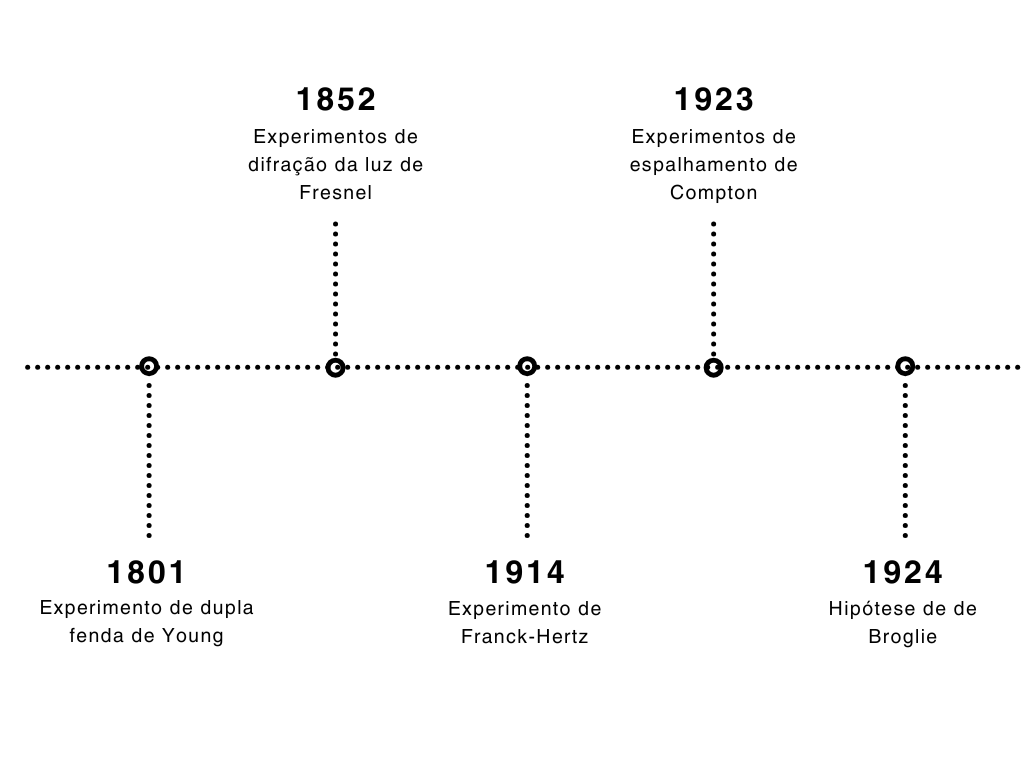
\includegraphics[width=0.75\textwidth,height=0.70\textheight,keepaspectratio]{figuras/linha o tempo.png}\par
        {\scriptsize Fonte: Elaborado pelo autor.}
        \end{figure}
        \end{center}
    
\end{frame}


\begin{frame}{Linha do tempo}
\centering
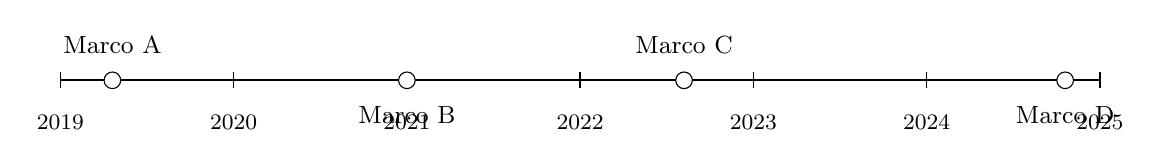
\begin{tikzpicture}[x=2.2cm, y=1cm, >=stealth,
    event/.style={circle, draw, fill=white, inner sep=1.5pt, minimum size=6pt},
    label above/.style={font=\small, align=center, above=6pt},
    label below/.style={font=\small, align=center, below=6pt}
]
  \draw[line width=0.6pt] (0,0) -- (6,0);
  \foreach \x/\txt in {0/2019,1/2020,2/2021,3/2022,4/2023,5/2024,6/2025}{
    \draw[line width=0.6pt] (\x,0.1) -- (\x,-0.1) node[below=6pt,font=\footnotesize] {\txt};
  }

  \node[event] (e1) at (0.3,0) {}; \node[label above] at (e1) {Marco A};
  \node[event] (e2) at (2.0,0) {}; \node[label below] at (e2) {Marco B};
  \node[event] (e3) at (3.6,0) {}; \node[label above] at (e3) {Marco C};
  \node[event] (e4) at (5.8,0) {}; \node[label below] at (e4) {Marco D};
\end{tikzpicture}
\end{frame}


\begin{frame}{Dualidade Onda-Partícula para Luz}

    \begin{columns}[c]
        \column{.45\textwidth}
        \begin{figure}
          \centering
          \caption{Albert Einstein}
          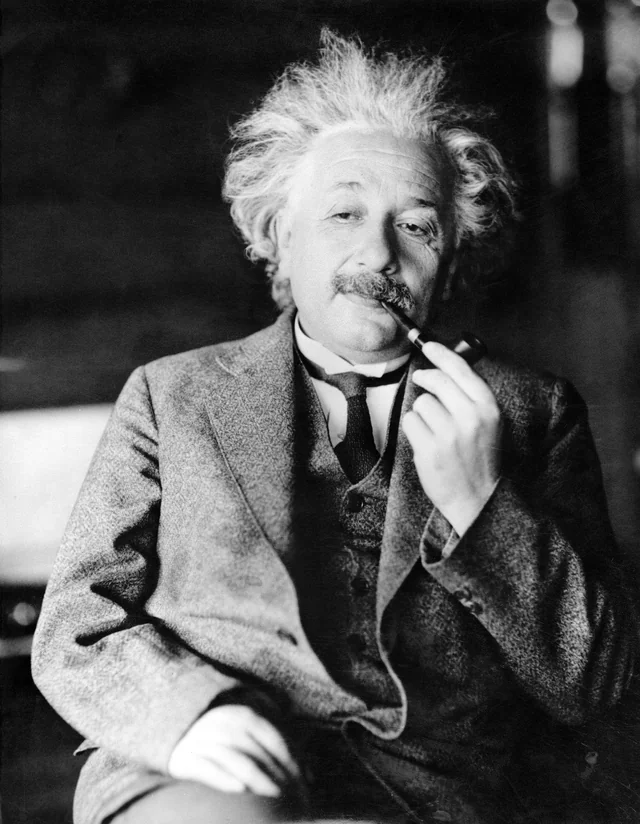
\includegraphics[width=4.25cm]{figuras/albert.png}\par
          {\scriptsize Fonte: Retirado da internet.}
        \end{figure}

        \column{.45\textwidth}
        Em \textbf{1905}, Albert Einstein apresenta o conceito de dualidade onda-partícula para a \textbf{luz} de forma a explicar o efeito fotoelétrico.

    \end{columns}

    
\end{frame}

%------------------------------------------------

\begin{frame}{Dualidade Onda-Partícula para Matéria}

    \begin{columns}[c]

        \column{.45\textwidth}
        \begin{figure}
          \centering
          \caption{Louis de Broglie}
          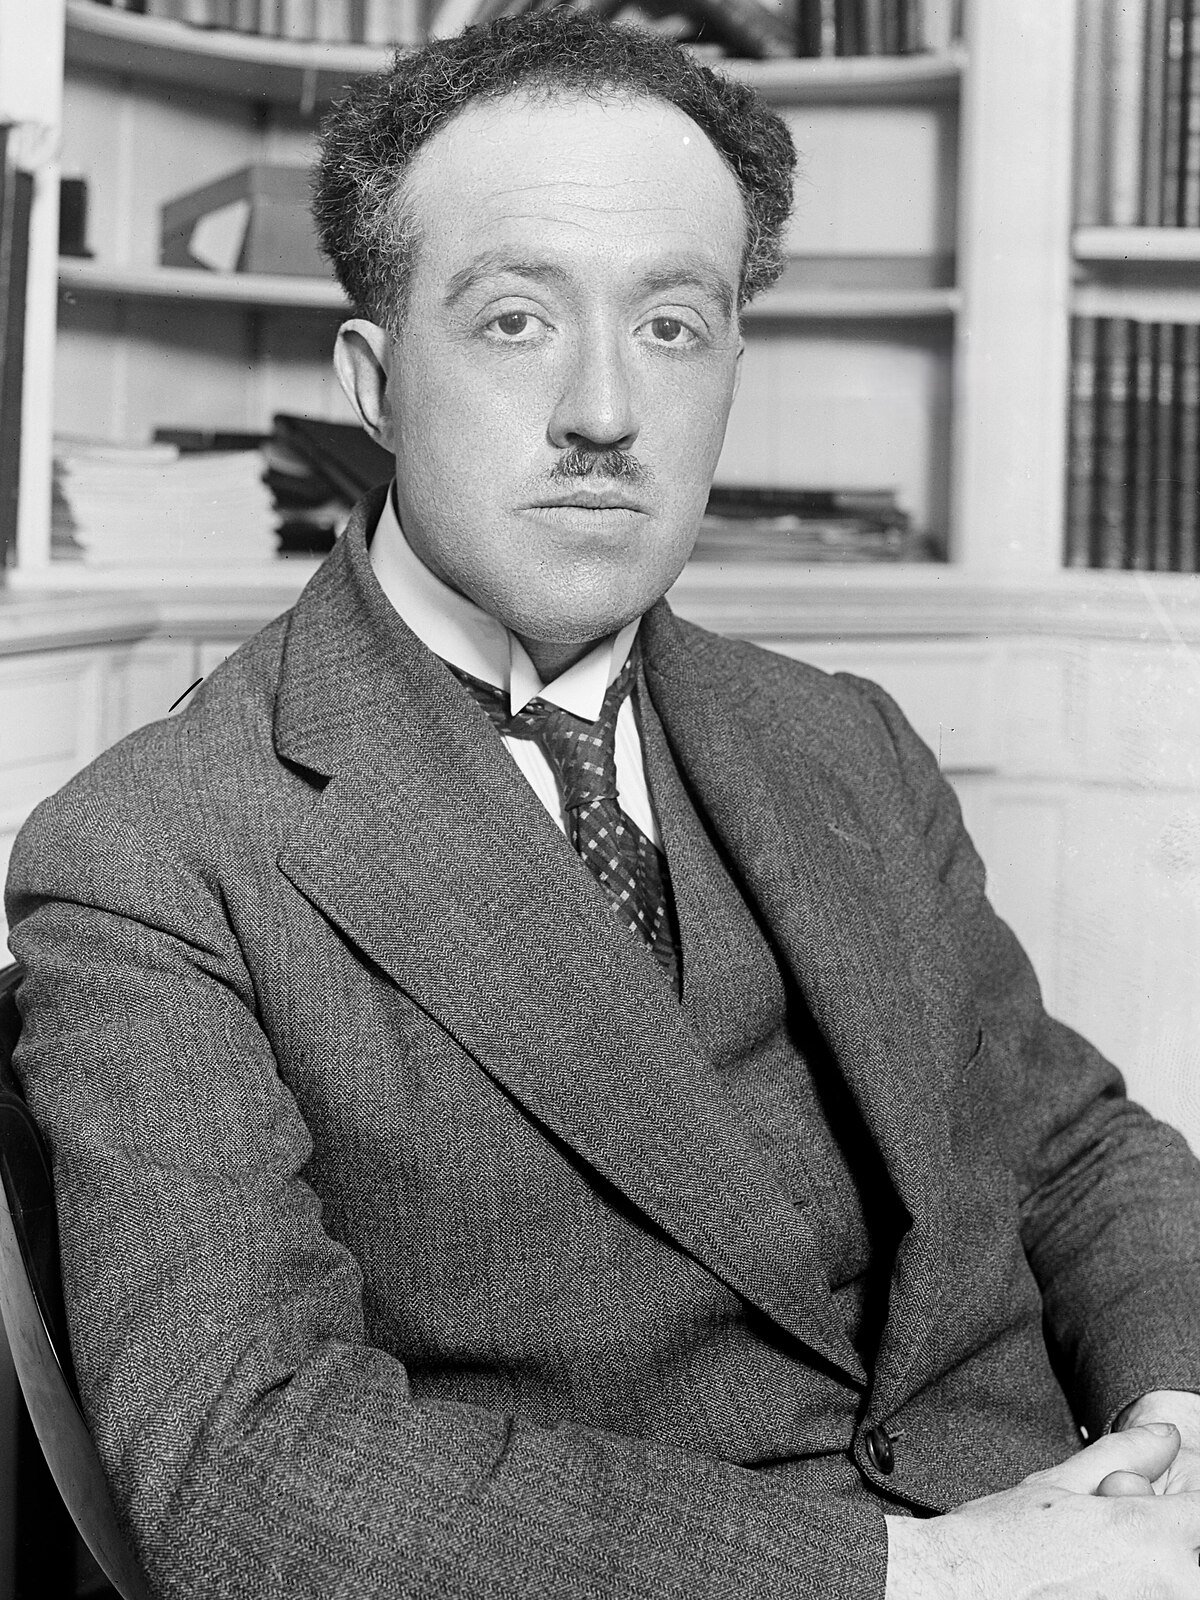
\includegraphics[width=4.25cm]{figuras/Prince_Louis-Victor_de_Broglie.jpg}\par
          {\scriptsize Fonte: Retirado da internet.}
        \end{figure}

        \column{.45\textwidth}
        Em \textbf{1924}, Louis de Broglie, em sua tese de doutorado, expande o conceito de dualidade onda-partícula para toda \textbf{matéria}.

    \end{columns}

\end{frame}
